% Artigo sobre o Q-BASIC (português).
% Compilar:  cd paper/artigo && latexmk -pdf main.tex
% Figuras, tabela e números: gerados por  python paper/gerar_figuras.py
\documentclass[11pt,a4paper]{article}

\usepackage[T1]{fontenc}
\usepackage[utf8]{inputenc}
\usepackage[english,brazil]{babel}
\usepackage{lmodern}
\usepackage{microtype}
\usepackage[margin=2.5cm]{geometry}
\usepackage{amsmath,amssymb}
\usepackage{braket}
\usepackage{icomma}
\usepackage{graphicx}
\usepackage{booktabs}
\usepackage{caption}
\usepackage[dvipsnames]{xcolor}
\usepackage{listings}
\usepackage{tikz}
\usetikzlibrary{arrows.meta,positioning}
\usepackage[numbers,sort&compress]{natbib}
\usepackage[colorlinks=true,linkcolor=Plum,citecolor=Plum,urlcolor=Plum]{hyperref}
\usepackage{xurl}

\graphicspath{{../figuras/}}
% Gerado por paper/gerar_figuras.py — não edite à mão.
\newcommand{\AmbienteNumpy}{2.5.4}
\newcommand{\AmbientePython}{3.13.18}
\newcommand{\AmbienteScipy}{1.18.1}
\newcommand{\ErroDOP}{1{,}9\times10^{-7}}
\newcommand{\ErroExpm}{2{,}1\times10^{-13}}
\newcommand{\ErroRK}{7{,}4\times10^{-7}}
\newcommand{\GanhoResolver}{177}
\newcommand{\GanhoSolver}{26}
\newcommand{\GanhoValorEsperado}{15}
\newcommand{\TempoDOP}{283}
\newcommand{\TempoExpm}{171}
\newcommand{\TempoRK}{827}
\newcommand{\TempoSolverAntes}{18{,}5}


\captionsetup{font=small,labelfont=bf}
\definecolor{roxoqb}{HTML}{5E17EB}
\definecolor{fundocodigo}{HTML}{F5F3FA}
\lstset{
  language=Python,
  basicstyle=\ttfamily\small,
  keywordstyle=\color{roxoqb}\bfseries,
  commentstyle=\color{gray}\itshape,
  stringstyle=\color{OliveGreen},
  backgroundcolor=\color{fundocodigo},
  frame=single,rulecolor=\color{black!15},
  columns=fullflexible,keepspaces=true,
  showstringspaces=false,
  xleftmargin=0.5em,xrightmargin=0.5em,
  aboveskip=0.8em,belowskip=0.8em,
  literate={á}{{\'a}}1 {é}{{\'e}}1 {í}{{\'i}}1 {ó}{{\'o}}1 {ú}{{\'u}}1
           {ã}{{\~a}}1 {õ}{{\~o}}1 {â}{{\^a}}1 {ê}{{\^e}}1 {ô}{{\^o}}1
           {ç}{{\c{c}}}1 {à}{{\`a}}1
}

\newcommand{\qbasic}{\textsc{Q-BASIC}}
\newcommand{\codigo}[1]{\texttt{#1}}

\title{\qbasic: um simulador quântico em Python para o ensino de óptica quântica
e computação quântica}
\author{Gubio Gomes de Lima\thanks{E-mail: \href{mailto:gubiofisikal@gmail.com}{gubiofisikal@gmail.com}}}
% TODO: incluir a afiliação do autor.
\date{}

\begin{document}

\maketitle

\begin{abstract}
\noindent
Apresentamos o \qbasic\ (\emph{Quantum Brazilian Algorithms, SImulations, and
Computational tools}), uma biblioteca de código aberto escrita em Python, sobre o NumPy e
o SciPy, voltada para o ensino de mecânica quântica, óptica quântica e computação
quântica. A biblioteca representa estados e operadores como matrizes densas ou esparsas e
oferece estados de Fock, coerentes e emaranhados; operadores de modos bosônicos e de
qubits; portas lógicas quânticas; a evolução temporal pelas equações de Schrödinger e de
Lindblad; grandezas como valores esperados, traço parcial, entropia de von Neumann e
fidelidade; e visualizações como a função de Wigner e a esfera de Bloch. O projeto nasceu
de uma sequência de aulas em que o simulador é construído do zero, e essa origem orienta
o seu desenho: interface em português, código curto e resultados verificáveis contra
soluções analíticas. Descrevemos os métodos numéricos e a arquitetura, mostramos
exemplos --- oscilações de Rabi, colapso e renascimento no modelo de Jaynes-Cummings,
decoerência de um estado do tipo gato de Schrödinger e teleportação quântica --- e
discutimos a validação e o desempenho.

\medskip
\noindent\textbf{Palavras-chave:} simulação quântica; óptica quântica; computação
quântica; ensino de física; Python.
\end{abstract}

\begin{otherlanguage}{english}
\begin{abstract}
\noindent
We present \qbasic\ (\emph{Quantum Brazilian Algorithms, SImulations, and Computational
tools}), an open-source Python library built on NumPy and SciPy for teaching quantum
mechanics, quantum optics and quantum computing. It represents states and operators as
dense or sparse matrices and provides Fock, coherent and entangled states, bosonic and
qubit operators, quantum logic gates, time evolution under the Schrödinger and Lindblad
equations, expectation values, partial traces, von Neumann entropy, fidelity, Wigner
functions and Bloch-sphere plots. The library grew out of a sequence of lessons in which
the simulator is built from scratch, which shapes its design: a Portuguese interface,
short readable code and results that can be checked against analytical solutions. We
describe the numerical methods and the architecture, show examples (Rabi oscillations,
collapse and revival in the Jaynes-Cummings model, decoherence of a Schrödinger-cat state
and quantum teleportation) and discuss validation and performance.

\medskip
\noindent\textbf{Keywords:} quantum simulation; quantum optics; quantum computing;
physics education; Python.
\end{abstract}
\end{otherlanguage}

% ===========================================================================
\section{Introdução}
% ===========================================================================

A simulação numérica é uma aliada natural do ensino de física quântica. Ela permite
explorar sistemas sem solução analítica simples, visualizar grandezas abstratas como a
função de Wigner e comparar, lado a lado, teoria e cálculo. Com a expansão das tecnologias
quânticas, essa ferramenta deixou de ser apenas um tópico de pós-graduação e passou a
fazer parte da formação de estudantes de física, engenharia e computação.

Existem bibliotecas maduras para esse fim. O QuTiP~\cite{johansson2012qutip,johansson2013qutip2}
é a referência em Python para óptica quântica e sistemas abertos; o
QuantumOptics.jl~\cite{kramer2018quantumoptics} cumpre papel semelhante em Julia; e o
Qiskit~\cite{javadi2024qiskit} é amplamente usado para circuitos quânticos. Essas
ferramentas são poderosas, mas o seu tamanho e as suas camadas de abstração (classes de
objetos, superoperadores, compiladores de circuitos, \emph{backends}) dificultam que um
estudante iniciante entenda o que acontece ``por dentro'' de um cálculo. Além disso, a
documentação e a interface são em inglês.

O \qbasic~\cite{qbasic2026} adota uma abordagem de ``caixa de vidro''. Ele nasceu de uma
sequência de aulas em notebooks Jupyter~\cite{kluyver2016jupyter} em que o estudante
programa, passo a passo, a representação matricial de estados e operadores, as operações
entre eles e a solução da equação de Schrödinger, comparando cada resultado com o
QuTiP. A biblioteca é a versão robusta desse mesmo código: as funções têm os nomes, em
português, que o estudante usou nas aulas, e a implementação de cada uma cabe em poucas
linhas sobre o NumPy~\cite{harris2020numpy} e o SciPy~\cite{virtanen2020scipy}. Ao mesmo
tempo, o projeto segue práticas profissionais de engenharia de software: testes
automatizados que verificam resultados físicos conhecidos, integração contínua,
documentação gerada a partir do código e publicação no PyPI.

Este artigo está organizado da seguinte forma. A seção~\ref{sec:fundamentos} resume os
fundamentos físicos e os métodos numéricos; a seção~\ref{sec:arquitetura} descreve a
arquitetura; a seção~\ref{sec:exemplos} apresenta exemplos; a
seção~\ref{sec:validacao} trata da validação e do desempenho; a
seção~\ref{sec:ensino} discute o uso no ensino; e a seção~\ref{sec:conclusao} conclui.

% ===========================================================================
\section{Fundamentos físicos e métodos numéricos}\label{sec:fundamentos}
% ===========================================================================

\subsection{Representação matricial e espaço de Fock truncado}

Estados são vetores coluna e operadores são matrizes numa base escolhida. Para um qubit,
usa-se a base computacional $\{\ket{0}, \ket{1}\}$. Para um modo do campo
eletromagnético (ou um oscilador harmônico), usa-se a base de Fock $\{\ket{n}\}$, que
precisa ser truncada em $N$ níveis. O operador de destruição é então a matriz
$N\times N$ com elementos $\braket{n-1|a|n} = \sqrt{n}$, e o truncamento tem uma
consequência que vale a pena discutir em sala: a relação de comutação canônica só vale
no subespaço que não toca o último nível,
\begin{equation}
  [a, a^\dagger] = I - N\ket{N-1}\bra{N-1}.
\end{equation}
Na prática, escolhe-se $N$ bem maior que os números de fótons relevantes --- para um
estado coerente $\ket{\alpha}$, alguns desvios-padrão acima de $|\alpha|^2$ --- e
verifica-se a convergência aumentando $N$.

Sistemas compostos são descritos pelo produto tensorial. No \qbasic, cada objeto guarda as
dimensões dos subsistemas (por exemplo, \codigo{[[2, 2], [1, 1]]} para um ket de dois
qubits), o que permite calcular o traço parcial sem que o usuário informe a estrutura. Os
qubits são numerados da esquerda para a direita: \codigo{ket("01")} representa
$\ket{0}\otimes\ket{1}$.

\subsection{Evolução de sistemas fechados}

Para um Hamiltoniano independente do tempo, a solução da equação de Schrödinger (com
$\hbar = 1$) é $\ket{\psi(t)} = e^{-iHt}\ket{\psi_0}$. O \qbasic\ calcula diretamente a
\emph{ação} da exponencial sobre o vetor com o algoritmo de Al-Mohy e
Higham~\cite{almohy2011expmv}, disponível no SciPy como \codigo{expm\_multiply}. O método
não forma a matriz $e^{-iHt}$, aceita matrizes esparsas e calcula, numa única chamada,
todos os instantes de uma grade uniforme; o erro fica na precisão de máquina. Como
alternativa, a equação diferencial pode ser integrada com os métodos de Runge-Kutta do
SciPy, como o de Dormand e Prince~\cite{dormand1980rk}.

\subsection{Sistemas abertos: a equação de Lindblad}

A dinâmica markoviana de um sistema aberto é descrita pela equação
mestra~\cite{lindblad1976,gorini1976}
\begin{equation}
  \frac{d\rho}{dt} = -i[H, \rho] + \sum_k \left( L_k \rho L_k^\dagger
  - \frac{1}{2}\left\{L_k^\dagger L_k, \rho\right\} \right),
  \label{eq:lindblad}
\end{equation}
em que os operadores de salto $L_k$ já incluem as taxas (por exemplo,
$L = \sqrt{\kappa}\,a$ para a perda de fótons de uma cavidade). Empilhando as colunas de
$\rho$ num vetor e usando $\mathrm{vec}(AXB) = (B^T \otimes A)\,\mathrm{vec}(X)$, a
equação~\eqref{eq:lindblad} vira $d\,\mathrm{vec}(\rho)/dt = \mathcal{L}\,\mathrm{vec}(\rho)$,
com o superoperador
\begin{equation}
  \mathcal{L} = -i\left(I \otimes H - H^T \otimes I\right)
  + \sum_k \left( L_k^* \otimes L_k - \tfrac{1}{2} I \otimes L_k^\dagger L_k
  - \tfrac{1}{2} (L_k^\dagger L_k)^T \otimes I \right).
\end{equation}
O \qbasic\ monta $\mathcal{L}$ como matriz esparsa $N^2 \times N^2$ e reutiliza o mesmo
evolutor da equação de Schrödinger. A forma explícita de $\mathcal{L}$ tem valor didático:
os seus autovalores são as taxas de relaxação do sistema.

\subsection{Função de Wigner}

A função de Wigner~\cite{wigner1932} pode ser escrita como o valor esperado do operador
paridade deslocado~\cite{cahill1969},
$W(\alpha) = \frac{2}{\pi}\mathrm{Tr}\left[\rho\, D(\alpha)\,\Pi\, D^\dagger(\alpha)\right]$,
com $\Pi = (-1)^{a^\dagger a}$. Na base de Fock, $W = \sum_{mn}\rho_{mn}W_{mn}$, e cada
termo tem forma fechada em polinômios de Laguerre generalizados; para $m \geq n$,
\begin{equation}
  W_{mn}(\alpha) = \frac{2}{\pi}(-1)^n \sqrt{\frac{n!}{m!}}\,(2\alpha^*)^{m-n}
  e^{-2|\alpha|^2} L_n^{(m-n)}\!\left(4|\alpha|^2\right),
\end{equation}
e $W_{nm} = W_{mn}^*$. O \qbasic\ usa essa expansão e devolve $W(x, p)$ nas quadraturas
$x = (a + a^\dagger)/\sqrt{2}$ e $p = -i(a - a^\dagger)/\sqrt{2}$, normalizada de modo
que $\int W\,dx\,dp = 1$. A implementação é testada contra a definição pela paridade
deslocada.

\subsection{Grandezas de informação quântica}

Para estados de sistemas compostos, a biblioteca calcula o traço parcial, a pureza
$\mathrm{Tr}\,\rho^2$, a entropia de von Neumann $S(\rho) = -\mathrm{Tr}\,\rho\log_2\rho$
(em bits) e a fidelidade de Uhlmann-Jozsa~\cite{uhlmann1976,jozsa1994},
$F(\rho,\sigma) = \left(\mathrm{Tr}\sqrt{\sqrt{\rho}\,\sigma\sqrt{\rho}}\right)^2$, que se
reduz a $|\braket{\psi|\phi}|^2$ para estados puros~\cite{nielsen2010}.

% ===========================================================================
\section{Arquitetura e implementação}\label{sec:arquitetura}
% ===========================================================================

A figura~\ref{fig:arquitetura} mostra a organização da biblioteca. Na base está a classe
\codigo{ObjQuantico}, que representa kets, bras, operadores e matrizes densidade. Os dados
ficam num \codigo{numpy.ndarray} (formato denso) ou num \codigo{scipy.sparse.csr\_array}
(formato esparso); os dois formatos podem ser misturados nas operações, e o resultado só
é esparso quando os dois operandos são. As convenções de operação, herdadas das aulas,
estão na tabela~\ref{tab:convencoes}.

\begin{figure}[htb]
  \centering
  \begin{tikzpicture}[
      caixa/.style={draw=roxoqb!80, fill=roxoqb!6, rounded corners=3pt, align=center,
        font=\small, minimum height=1.05cm, inner sep=4pt},
      seta/.style={-{Stealth[length=2mm]}, draw=black!55}]
    \node[caixa, minimum width=12.6cm] (objeto) at (0,0)
      {\texttt{objeto}: \texttt{ObjQuantico} --- denso (NumPy) ou esparso (SciPy), \texttt{dims}, aritmética};
    \node[caixa, minimum width=4cm] (estados) at (-4.3,1.7) {\texttt{estados}\\Fock, coerente, Bell, GHZ, $\rho$};
    \node[caixa, minimum width=4cm] (operadores) at (0,1.7) {\texttt{operadores}\\$a$, $a^\dagger$, $x$, $p$, Pauli, $\otimes$};
    \node[caixa, minimum width=4cm] (portas) at (4.3,1.7) {\texttt{portas}\\H, S, T, $R_{x,y,z}$, CNOT};
    \node[caixa, minimum width=6.1cm] (medidas) at (-3.25,3.4) {\texttt{medidas}\\$\langle O\rangle$, traço parcial, $S$, $F$, Bloch};
    \node[caixa, minimum width=6.1cm] (dinamica) at (3.25,3.4) {\texttt{dinamica}\\Schrödinger e Lindblad};
    \node[caixa, minimum width=12.6cm] (visual) at (0,5.1) {\texttt{visualizacao}: função de Wigner, esfera de Bloch, gráficos (matplotlib)};
    \foreach \no in {estados, operadores, portas} \draw[seta] (objeto) -- (\no);
    \draw[seta] (estados) -- (medidas);
    \draw[seta] (operadores) -- (dinamica);
    \draw[seta] (medidas) -- (dinamica);
    \draw[seta] (medidas) -- (visual);
    \draw[seta] (dinamica) -- (visual);
  \end{tikzpicture}
  \caption{Módulos do \qbasic. As setas indicam dependência: tudo é construído sobre a
  classe \texttt{ObjQuantico}.}
  \label{fig:arquitetura}
\end{figure}

\begin{table}[htb]
  \centering
  \caption{Convenções das operações com objetos quânticos.}
  \label{tab:convencoes}
  \small
  \begin{tabular}{ll}
    \toprule
    Expressão & Significado \\
    \midrule
    \texttt{A * B} & produto matricial (operador $\times$ operador, operador $\times$ ket, bra $\times$ ket) \\
    \texttt{A @ B}, \texttt{tensor(A, B)} & produto tensorial $A\otimes B$ \\
    \texttt{c * A}, \texttt{A / c} & multiplicação e divisão por um número complexo \\
    \texttt{A + c} & $A + c\,I$ \\
    \texttt{A.dag()}, \texttt{A ** n} & adjunto $A^\dagger$ e potência inteira \\
    \bottomrule
  \end{tabular}
\end{table}

Sobre essa classe, os módulos \codigo{estados}, \codigo{operadores} e \codigo{portas}
constroem os objetos físicos; \codigo{medidas} calcula valores esperados, probabilidades,
amostras de medidas e grandezas de informação quântica; \codigo{dinamica} resolve as
equações de Schrödinger e de Lindblad, devolvendo os estados e os valores esperados em
cada instante; e \codigo{visualizacao} produz a função de Wigner e os gráficos com o
matplotlib~\cite{hunter2007matplotlib}. As portas de muitos qubits são construídas por uma
permutação: para aplicar uma porta $U$ de $k$ qubits aos qubits de índices quaisquer de
um registro, monta-se a matriz de permutação $P$ que leva esses qubits para o início e
calcula-se $P^T (U \otimes I) P$. Assim, CNOTs entre qubits não vizinhos, Toffoli e
portas controladas genéricas usam o mesmo código.

O projeto adota práticas de engenharia de software comuns em bibliotecas científicas: o
código é empacotado com \codigo{pyproject.toml} e publicado no PyPI; mais de 800 testes
automatizados (cobertura de 98\,\%) rodam a cada alteração no GitHub Actions, em Linux,
Windows e macOS, e com Python de 3.10 a 3.14; os exemplos das docstrings e todos os
notebooks dos tutoriais também são executados; e a documentação, com a referência de todas
as funções, é gerada a partir do código. Os nomes das versões anteriores continuam
funcionando, com avisos que indicam o nome novo.

% ===========================================================================
\section{Exemplos}\label{sec:exemplos}
% ===========================================================================

\subsection{Oscilação de Rabi}

O exemplo mínimo de dinâmica é um qubit sob $H = (\Omega/2)\,\sigma_x$, para o qual
$\braket{\sigma_z}(t) = \cos(\Omega t)$. Com $\Omega = 1$:

\begin{lstlisting}
import numpy as np
import qbasic as qb

tempos = np.linspace(0, 4 * np.pi, 25)
H = 0.5 * qb.pauliX()
res = qb.resolver_schrodinger(H, qb.ket("0"), tempos,
                              observaveis=[qb.pauliZ()])
z = res.valores_esperados[0]          # igual a np.cos(tempos)
\end{lstlisting}

\noindent O resultado está na figura~\ref{fig:dinamica}(a). O código lê como a física:
o Hamiltoniano é escrito como na lousa, e o estado inicial e o observável são passados
explicitamente.

\begin{figure}[htb]
  \centering
  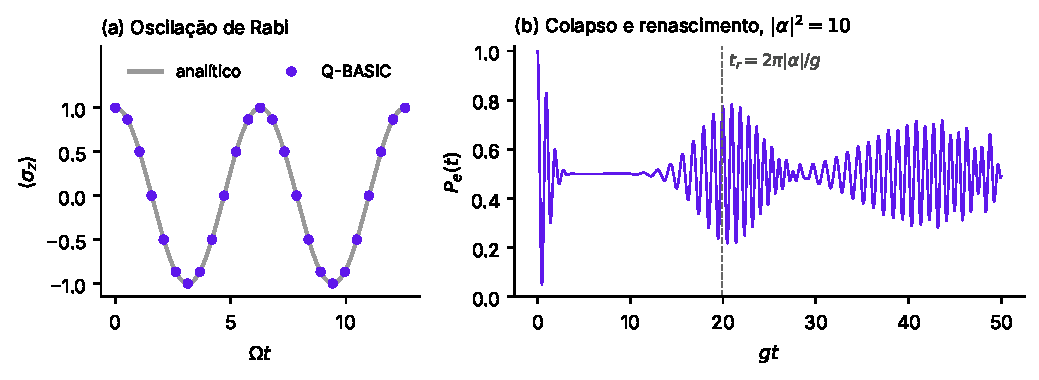
\includegraphics[width=\linewidth]{fig_dinamica.pdf}
  \caption{(a) Oscilação de Rabi de um qubit: solução analítica (linha) e \qbasic\ (pontos).
  (b) Probabilidade de o átomo estar excitado no modelo de Jaynes-Cummings com a cavidade
  num estado coerente com $|\alpha|^2 = 10$ ($N = 40$ níveis de Fock): colapso das
  oscilações e renascimento próximo de $t_r = 2\pi|\alpha|/g$ (linha tracejada).}
  \label{fig:dinamica}
\end{figure}

\subsection{Colapso e renascimento no modelo de Jaynes-Cummings}

O modelo de Jaynes-Cummings~\cite{jaynes1963} descreve um átomo de dois níveis acoplado a
um modo de cavidade. Em ressonância e no referencial que gira com a frequência comum,
$H = g\,(a^\dagger\sigma_- + a\,\sigma_+)$. Com o átomo excitado e a cavidade num estado
coerente, a probabilidade de excitação é
\begin{equation}
  P_e(t) = \sum_n p_n \cos^2\!\left(g\sqrt{n+1}\,t\right), \qquad
  p_n = e^{-|\alpha|^2}\frac{|\alpha|^{2n}}{n!}.
\end{equation}
As oscilações com frequências diferentes se desfazem rapidamente (colapso) e voltam a
entrar em fase em $t_r \approx 2\pi|\alpha|/g$ (renascimento), um efeito sem análogo
clássico, ligado ao caráter discreto do campo~\cite{eberly1980,gerry2005}. Com operadores
esparsos:

\begin{lstlisting}
N, g, alfa = 40, 1.0, np.sqrt(10)
a  = qb.tensor(qb.destruicao(N, sparsa=True), qb.identidade(2, sparsa=True))
sm = qb.tensor(qb.identidade(N, sparsa=True), qb.destruicao(2, sparsa=True))
H  = g * (a.dag() * sm + a * sm.dag())

psi0 = qb.tensor(qb.coerente(N, alfa), qb.ket("1"))   # átomo excitado
res  = qb.resolver_schrodinger(H, psi0, np.linspace(0, 50, 1500),
                               observaveis=[sm.dag() * sm])
\end{lstlisting}

\noindent A figura~\ref{fig:dinamica}(b) mostra o resultado. O mesmo \codigo{res} permite
estudar o emaranhamento entre átomo e cavidade: \codigo{qb.entropia\_von\_neumann(qb.traco\_parcial(psi, 1))}
dá a entropia do átomo em cada instante.

\subsection{Decoerência de um gato de Schrödinger}

Um estado do tipo gato de Schrödinger, $\ket{\alpha} + \ket{-\alpha}$ (normalizado),
tem franjas de interferência com valores negativos na função de Wigner. Quando a
cavidade perde fótons com taxa $\kappa$, as coerências entre as duas componentes decaem
com taxa da ordem de $2\kappa|\alpha|^2$ --- muito mais depressa que a energia do
campo~\cite{haroche2006}. Com a equação de Lindblad:

\begin{lstlisting}
N, alfa = 30, 2.0
a = qb.destruicao(N)
gato = (qb.coerente(N, alfa) + qb.coerente(N, -alfa)).normalizar()
res = qb.resolver_lindblad(0 * qb.numero(N), gato, [0, 0.1, 0.4], [a])  # kappa = 1
x = np.linspace(-4.5, 4.5, 241)
W = [qb.wigner(rho, x, x) for rho in res.estados]
\end{lstlisting}

\noindent A figura~\ref{fig:wigner} mostra a perda das franjas: em $\kappa t = 0{,}1$ elas
já perderam boa parte do contraste e, em $\kappa t = 0{,}4$, restam apenas as duas
gaussianas de uma mistura estatística, com pureza próxima de $1/2$.

\begin{figure}[htb]
  \centering
  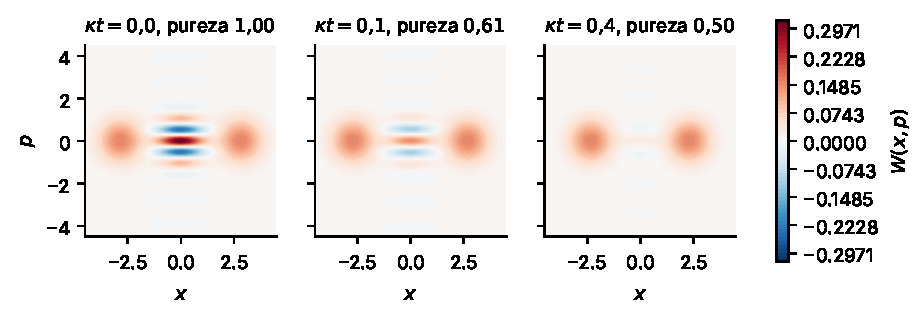
\includegraphics[width=\linewidth]{fig_wigner.pdf}
  \caption{Função de Wigner de um gato de Schrödinger com $\alpha = 2$ sob perda de
  fótons, em três instantes. As franjas de interferência (valores negativos, em azul)
  desaparecem muito antes das duas componentes coerentes.}
  \label{fig:wigner}
\end{figure}

\subsection{Circuitos quânticos: estado de Bell e teleportação}

Para circuitos, as portas são operadores comuns, e o circuito é o seu produto (da direita
para a esquerda). O protocolo de teleportação~\cite{bennett1993,nielsen2010} pode ser
simulado com as correções clássicas substituídas por portas controladas (princípio da
medida adiada):

\begin{lstlisting}
psi = qb.rz(0.7) * qb.ry(1.1) * qb.ket("0")          # estado a teleportar
estado = qb.tensor(psi, qb.bell("phi+"))             # qubits 1 e 2: par de Bell
estado = qb.cnot(0, 1, n_qubits=3) * estado
estado = qb.porta_em(qb.hadamard(), 0, 3) * estado
estado = qb.cnot(1, 2, n_qubits=3) * estado          # correção X
estado = qb.cz(0, 2, n_qubits=3) * estado            # correção Z
qb.fidelidade(qb.traco_parcial(estado, 2), psi)      # 1.0
\end{lstlisting}

\noindent A fidelidade igual a 1 entre o estado do qubit 2 e o estado original confirma
o protocolo. A função \codigo{qb.amostrar} simula medidas repetidas na base computacional,
como num processador quântico real.

% ===========================================================================
\section{Validação e desempenho}\label{sec:validacao}
% ===========================================================================

\subsection{Testes contra resultados conhecidos}

Os testes automatizados verificam propriedades físicas, e não detalhes de implementação:
a álgebra das matrizes de Pauli, $a\ket{n} = \sqrt{n}\ket{n-1}$, $[x, p] = i$ (a menos do
truncamento), a distribuição de Poisson do estado coerente, as oscilações de Rabi, a
dinâmica de Jaynes-Cummings comparada com a diagonalização exata, a emissão espontânea
($P_e = e^{-\gamma t}$), o oscilador amortecido, a tabela-verdade das portas e a função de
Wigner do vácuo, de estados de Fock e de estados coerentes. Quase todos os testes rodam
duas vezes, com matrizes densas e esparsas, garantindo que os dois formatos dão o mesmo
resultado.

\subsection{Precisão dos métodos de evolução}

A figura~\ref{fig:precisao} compara os métodos de evolução no modelo de Jaynes-Cummings
com campo coerente ($|\alpha|^2 = 10$, dimensão 80) em relação à diagonalização exata.
O método padrão, \codigo{expm}, tem erro máximo de $\ErroExpm$, contra $\ErroDOP$ do
DOP853 e $\ErroRK$ do RK45 (ambos com tolerâncias $\mathrm{rtol} = 10^{-8}$ e
$\mathrm{atol} = 10^{-10}$), e foi também o mais rápido nesse caso ($\TempoExpm$\,ms,
contra $\TempoDOP$\,ms e $\TempoRK$\,ms). Os integradores de Runge-Kutta continuam úteis
quando o estado ocupa um subespaço pequeno de um espaço grande, situação em que o
controle adaptativo do passo é vantajoso.

\begin{figure}[htb]
  \centering
  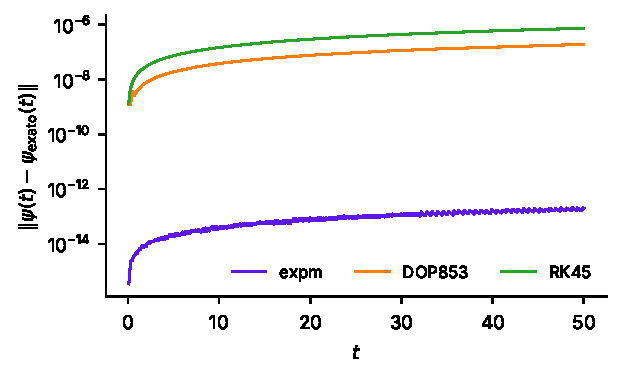
\includegraphics[width=0.62\linewidth]{fig_precisao.pdf}
  \caption{Erro $\|\psi(t) - \psi_\text{exato}(t)\|$ dos métodos de evolução no modelo de
  Jaynes-Cummings com campo coerente.}
  \label{fig:precisao}
\end{figure}

\subsection{Desempenho}

A tabela~\ref{tab:desempenho} e a figura~\ref{fig:desempenho} comparam a versão atual com a
versão anterior à reestruturação da biblioteca, nas mesmas operações e no mesmo
computador (Python \AmbientePython, NumPy \AmbienteNumpy, SciPy \AmbienteScipy). Os
ganhos vêm de escolhas simples: o valor esperado ao longo do tempo é calculado de uma vez
com \codigo{numpy.einsum}, em vez de um laço em Python
(${\sim}\GanhoValorEsperado\times$); o integrador deixou de converter o Hamiltoniano
esparso em denso (${\sim}\GanhoSolver\times$); as potências usam exponenciação binária; e a
exibição dos objetos não depende mais da conversão para o SymPy. No caso mais custoso, a
evolução do modelo de Jaynes-Cummings com dimensão 400, a versão anterior levava
$\TempoSolverAntes$\,s, e a evolução exata com \codigo{resolver\_schrodinger} é cerca de
$\GanhoResolver$ vezes mais rápida.

\begin{table}[htb]
  \centering
  \caption{Tempo das operações antes e depois da reestruturação (menor de três repetições).
  $^*$Em relação ao integrador da versão anterior no mesmo sistema.}
  \label{tab:desempenho}
  \small
  \begin{tabular}{lrrr}
\toprule
Operação & Antes (ms) & Depois (ms) & Ganho \\
\midrule
Valor esperado (2000 instantes) & 160,98 & 10,45 & 15,4\\
Potência $x^{64}$ (denso 200×200) & 10,75 & 1,41 & 7,6\\
Montar $H$ esparso ($N = 2000$) & 3,10 & 1,97 & 1,6\\
Solver, $H$ esparso (dimensão 400) & 18.472,50 & 703,71 & 26,3\\
Estado coerente (analítico) & 0,03 & 0,02 & 1,3\\
repr() (40×40) & 10,68 & 0,13 & 81,8\\
\texttt{resolver\_schrodinger} (exato), mesmo sistema & --- & 104,34 & 177$^*$\\
\bottomrule
\end{tabular}

\end{table}

\begin{figure}[htb]
  \centering
  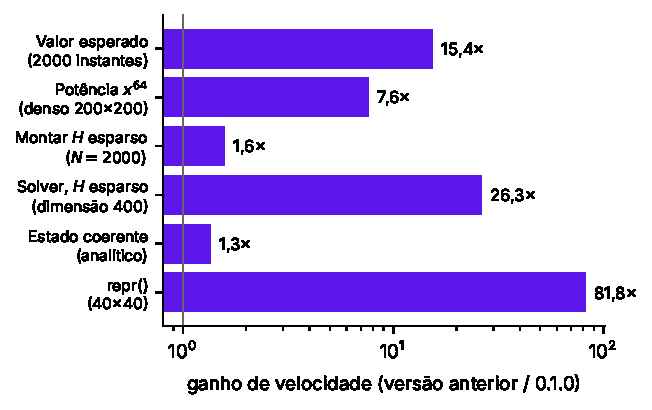
\includegraphics[width=0.62\linewidth]{fig_desempenho.pdf}
  \caption{Ganho de velocidade da versão 0.1.0 em relação à versão anterior (escala
  logarítmica).}
  \label{fig:desempenho}
\end{figure}

% ===========================================================================
\section{Uso no ensino}\label{sec:ensino}
% ===========================================================================

O material didático do \qbasic\ é uma sequência de notebooks (tabela~\ref{tab:aulas}). Na
primeira parte, o estudante constrói o simulador: representa kets e operadores, implementa
as operações, gera estados coerentes por dois caminhos (operador deslocamento e fórmula
fechada), monta Hamiltonianos de sistemas acoplados e resolve a equação de Schrödinger,
sempre comparando com o QuTiP. As aulas finais usam a biblioteca pronta para temas mais
avançados. A segunda parte trata de computação quântica. Os mesmos notebooks são
publicados no site da documentação e reunidos automaticamente num livro em PDF, de modo
que o material impresso, o site e os notebooks nunca divergem.

\begin{table}[htb]
  \centering
  \caption{Sequência de tutoriais.}
  \label{tab:aulas}
  \small
  \begin{tabular}{lp{11.5cm}}
    \toprule
    Aula & Conteúdo \\
    \midrule
    0 & Kets, bras, operadores, estado de Fock e matriz densidade (com o QuTiP) \\
    1--3 & A classe de objetos quânticos e as operações: soma, produtos interno, externo,
           matricial e tensorial \\
    4--7 & Matrizes de Pauli, estado coerente, matriz densidade, operadores posição e momento \\
    8--9 & Hamiltonianos de sistemas acoplados e solução da equação de Schrödinger \\
    10--11 & A biblioteca \qbasic\ e a versão com matrizes esparsas \\
    12 & Função de Wigner, colapso e renascimento, emaranhamento e equação de Lindblad \\
    \midrule
    CQ 1 & Estados, superposição, medida e um simulador de qubits com o NumPy \\
    CQ 2 & Esfera de Bloch, portas, medidas, estado de Bell, GHZ e W, teleportação \\
    \bottomrule
  \end{tabular}
\end{table}

Algumas atividades que o material favorece são: comparar as soluções numérica e analítica
da oscilação de Rabi; estudar a convergência dos resultados com o número $N$ de níveis de
Fock; observar como a precisão dos integradores depende das tolerâncias; e relacionar a
perda de pureza com o desaparecimento das franjas da função de Wigner. Como o código de
cada função é curto e escrito em português, o estudante pode ler a implementação da
biblioteca e reconhecê-la como a versão final do que programou nas aulas.

% ===========================================================================
\section{Conclusões e perspectivas}\label{sec:conclusao}
% ===========================================================================

O \qbasic\ é uma biblioteca de simulação quântica pensada para o ensino, que cobre de
estados e operadores básicos a sistemas abertos e circuitos quânticos, com uma interface em
português e uma implementação curta e verificável. A sua origem numa sequência de aulas em
que o simulador é construído do zero faz dele uma ``caixa de vidro'': o estudante sabe o
que cada função faz porque já a programou. Ao mesmo tempo, a biblioteca é rápida o
bastante para os sistemas usados em sala e em projetos de iniciação científica, e é
mantida com testes automatizados e documentação.

Os próximos passos incluem Hamiltonianos dependentes do tempo, algoritmos quânticos
clássicos (Deutsch-Jozsa, Grover e a transformada de Fourier quântica) como tutoriais,
implementações para GPU com o PyTorch e o CuPy, e uma versão da documentação em inglês.

\section*{Disponibilidade}

O \qbasic\ é software livre (licença MIT). O código está em
\url{https://github.com/GubioGL/Q-BASIC}; a instalação é feita com
\codigo{pip install Q-BASIC}; e a documentação, com os tutoriais, está em
\url{https://gubiogl.github.io/Q-BASIC/}. As figuras e os números deste artigo são gerados
pelo script \codigo{paper/gerar\_figuras.py} do repositório.

% TODO: \section*{Agradecimentos}

\bibliographystyle{unsrtnat}
\bibliography{referencias}

\end{document}
